
\documentclass{article}

\usepackage[]{todonotes}
\usepackage[outdir=./]{epstopdf}
\usepackage[ruled]{algorithm2e}

\title{Parallel Standard Particle Swarm Optimization}
\author{Gian M. Fritsche}
\date{\today}

\begin{document}
    \maketitle

    \section{Introduction}

    The Particle Swarm Optimization~\cite{PSO95} is a meta-heuristic based on the behavior of bird flocks. Every iteration, each particle moves in the search space based on three components:

    \begin{itemize}
        \item {\em Social:} This component contributes for the exploitation of the algorithm.
        It guides the search towards the best solutions found by the swarm.
        \item {\em Individual:} The individual component guides the particle to the best region that the particle has found.
        \item {\em Inertia:} The inertia component increase the exploration of the algorithm. It is responsible for keeping the particle moving towards a previous direction and avoid abrupt changes of direction.
    \end{itemize}

    The position of one particle is a set of variable values, {\em i.e.} a solution for an optimization problem. Then, the algorithms evaluate the solution, and a fitness value is associated. Based on the fitness value the Social and Individual components are updated.
    Moreover, these components are used to compute the next position of the particle (another solution for the problem).

    Since its first publication, the PSO had proposed several adaptations and improvements.
    In 2006 it was created the first version of a Standard Particle Swarm Optimization~\cite{SPSO}. The SPSO was not proposed to be the best PSO available, but establish a common benchmark as a baseline to assess the PSO variants in the literature.

    \subsection {Standard Particle Swarm optimization}

    Since its first publication (2006), there is three versions of SPSO: 2006, 2007 and 2011.
    In the latest version the description is given as follow (and showed in Algorithm~\ref{alg:spso2011}):
    The first population (set of solutions) is initialized randomly in the search space. Then, the algorithms initialize the velocity also randomly. The suggested population size is $40$. The neighborhood topology used to update the social component is the Adaptive Random Topology (ART).
    In the ART each particle informs its current fitness to $K$ neighbors. If the fitness is better than the previous social best information of the neighbor the social best (fitness and position) is updated. A direct graph represents the neighborhood, where each particle informs its quality to (at most) $K$ neighbors. The graph is generated randomly initially and every time that the best global fitness is not improved.

    In the previous versions of PSO, the velocity was updated dimension by dimension.
    However, in SPSO2011 the velocity is updated in a geometrical way,  that does not depend on the system of coordinates.

    \begin{algorithm}[!htb]
        \KwResult{The best solution and its fitness}
        
        create adaptive random neighbourhood\;

        \ForEach{particle $ i \in swarm$}{
            initialize particles' position ($\vec{X_i}$) and velocity ($\vec{V_i}$)\;
            evaluate particle ($f(\vec{X_i})$)\;
            initialize personal best ($\vec{P_i}$) and neighbour best ($\vec{G_i}$)\;
            update global best fitness ($best\_fitness=\min(f(\vec{X_i}), best\_fitness)$)\;
        }
        number of iterations ($T$) = 1\;
        \While{$T < MAX\_IT$  }{
            $previous\_best\_fitness = best\_fitness$\;
            \ForEach{particle $ i \in swarm$}{
                update particle's velocity ($\vec{V_i}$)\;
                update particle's position ($\vec{X_i}$)\;
                evaluate particle ($f(\vec{X_i})$)\;
                \If{ $f(\vec{X_i}) < f(\vec{P_i})$ }{
                    $\vec{P_i} = \vec{X_i}$\;
                }
                update neighbour best ($\vec{G_i}$)\;
                update global best fitness ($best\_fitness=\min(f(\vec{X_i}), best\_fitness)$)\;
            }
            \If{$previous\_best\_fitness \le best\_fitness$}{
                create adaptive random neighbourhood\;
            }

            $T=T+1$
        }
        \ForEach{particle $ i \in swarm$}{
            \If{$f(\vec{X_i}) == best\_fitness$}{
                $best\_solution = \vec{X_i}$\; 
            }
        }
        
        \caption{Standard Particle Swarm Optimization 2011}
        \label{alg:spso2011}
    \end{algorithm}

    \section{Parallel SPSO-2011}

    \subsection{Related works}

    In the literature, it is possible to find different proposals of Parallel PSOs.
    One of the most recent is the GPU-based Asynchronous Particle Swarm Optimization~\cite{GPUPSO}.
      That implements a simple ring topology.
      In~\cite{ReviewGPUPSO}, it is presented a review of Particle Swarm Optimization on GPU.
      The paper presents 28 references of PSO on GPU including multi-objective versions and variations of PSO from 2009 to 2014.
      One of the papers from the review implements the Standard Particle Swarm Optimization 2007 using GPU~\cite{GPUSPSO2007}. The GPU version was 11 times faster than the CPU, mainly with a large population and high dimensional problems.

      \subsection{Proposal}

    In this work, we use the SPSO2011, which uses the Adaptive Random Neighborhood topology.  
    During the literature review, it was not found any other implementation of the SPSO2011 using GPU.
    The parallel implementation associates each particle with one thread (Algorithm~\ref{alg:pspso2011}).
    In this way, all \texttt{{\bf foreach} particle $ i \in swarm$ } were removed and executed in parallel based on the thread id inside the block ($threadIdx.x$ or $tid$).
    In the create adaptive random neighborhood method each particle selects up to $K$ neighbors. Then the particle updates its position and velocity; the position is evaluated using the fitness function, and the personal best is updated.
    Then, to update the neighbor best information, the particle search on the adjacency matrix of the neighborhood for all its neighbors and compares to itself.
    The best global fitness is computed using atomic operations. The $atomicMin(a, b)$ was implemented based on the CUDA $atomicCAS$, which realizes a compare and swap operation.
    Before entering the main loop, the implementation applies a thread synchronization.

    The first particle copies the best fitness for later comparison.
    Inside the main loop, the particle updates its velocity, position, and fitness.
    The personal best information is updated.
    Before set the neighbor best information a synchronization is necessary because the threads must compare its fitness to the updated value of its neighbors.
    Then, the neighbor best information is updated. Also, the best fitness is updated using the $atomicMin$ function.
    After the best fitness update it is applied another \texttt{\_\_syncthreads()}. To wait for all threads update the best fitness before using its value.
    If the best fitness is not improved, then the new neighborhood matrix is generated.
    After $T$ iterations the solution with fitness equals to the best fitness is the output of the algorithm.

    \begin{algorithm}[!htb]
        \KwResult{The best solution and its fitness}
        
        $tid = threadIdx.x\;$

        create adaptive random neighbourhood\;
        \_\_syncthreads()\;

        initialize particles' position ($\vec{X_{tid}}$) and velocity ($\vec{V_{tid}}$)\;
        evaluate particle ($f(\vec{X_{tid}})$)\;
        initialize personal best ($\vec{P_{tid}}$) and neighbour best ($\vec{G_{tid}}$)\;
        \tcc{the update global best uses atomicMin operation}
        update global best fitness ($best\_fitness=\min(f(\vec{X_{tid}}), best\_fitness)$)\;
        \_\_syncthreads()\;
        number of iterations ($T$) = 1\;
        \While{$T < MAX\_IT$  }{
            \If{$tid == 0$}{
                $previous\_best\_fitness = best\_fitness$\;
            }
            
            update particle's velocity ($\vec{V_{tid}}$)\;
            update particle's position ($\vec{X_{tid}}$)\;
            evaluate particle ($f(\vec{X_{tid}})$)\;
            \If{ $f(\vec{X_{tid}}) < f(\vec{P_{tid}})$ }{
                $\vec{P_{tid}} = \vec{X_{tid}}$\;
            }
            \_\_syncthreads()\;
            update neighbour best ($\vec{G_{tid}}$)\;
            \tcc{the update global best uses atomicMin operation}
            update global best fitness ($best\_fitness=\min(f(\vec{X_{tid}}), best\_fitness)$)\;
            \_\_syncthreads()\;
            
            \If{$previous\_best\_fitness \le best\_fitness$}{
                create adaptive random neighbourhood\;
            }

            $T=T+1$
        }
        
        \If{$f(\vec{X_{tid}}) == best\_fitness$}{
            $best\_solution = \vec{X_{tid}}$\; 
        }
        
        \caption{Parallel Standard Particle Swarm Optimization 2011}
        \label{alg:pspso2011}
    \end{algorithm}

    In the first implemented version it was not used shared memory, but in a second implementation it was used and the execution time was improved.
    Another item important to highlight is the two \texttt{\_\_syncthreads()} inside the loop.
    The use of \texttt{\_\_syncthreads()} generally slow down the execution of a CUDA program.
    However, in this implementation we did not have this problem due to the block size equals to warp size.
    Since the threads in the same warp execute in true (hardware) parallelism, there is no situation where threads need to sync with others on the same block.

    The first experiments were executed using only one block. However, the experiments run the SPSO several times; those executions can be run in parallel, using different and independent blocks. In the experiments using only one block the CPU implementation had a better execution time. However, when using multi executions at once, the GPU implementation achieved a better execution time.
    The next section details the experiments and results.

    \section{Experiments and Results}

    The first experiment was used to validate the equivalence regarding the quality of the GPU and CPU implementation. Both implementations showed similar convergence along the execution.

    For this, and all other, experiment it was used $T=3125$ iterations, $32$ particles, $D=10$ decision variables, $K=3$, and the Sphere function for fitness evaluation.  We executed $51$ independent runs. Those parameters were based on~\cite{SPSOCEC}. Moreover, the Sphere function is a simple optimization function present on the COCO (Comparing Continuous Optimisers) benchmark~\footnote{http://coco.gforge.inria.fr/}.

    The Table~\ref{tbl:gpuinfo} presents the information about the used GPU.
    Besides, the Table~\ref{tbl:cpuinfo} presents the CPU information.

    \begin{table}[!htb]
        \centering
        \caption{GPU information}
        \label{tbl:gpuinfo}
        \begin{tabular}{|l|l|}
            \hline
            \multicolumn{2}{|c|}{\textbf{--- General Information for device 0 ---}} \\ \hline
            \textbf{Name}                          & GeForce GTX 680                \\ \hline
            \textbf{Compute capability}            & 3.0                            \\ \hline
            \textbf{Clock rate}                    & 1058500                        \\ \hline
            \textbf{Device copy overlap}           & Enabled                        \\ \hline
            \textbf{Kernel execution timeout}      & Disabled                       \\ \hline
            \multicolumn{2}{|c|}{\textbf{--- Memory Information for device 0 ---}}  \\ \hline
            \textbf{Total global mem}              & 2095382528                     \\ \hline
            \textbf{Total constant Mem}            & 65536                          \\ \hline
            \textbf{Max mem pitch}                 & 2147483647                     \\ \hline
            \textbf{Texture Alignment}             & 512                            \\ \hline
            \multicolumn{2}{|c|}{\textbf{--- MP Information for device 0 ---}}      \\ \hline
            \textbf{Multiprocessor count}          & 8                              \\ \hline
            \textbf{Shared mem per mp}             & 49152                          \\ \hline
            \textbf{Registers per mp}              & 65536                          \\ \hline
            \textbf{Threads in warp}               & 32                             \\ \hline
            \textbf{Max threads per block}         & 1024                           \\ \hline
            \textbf{Max thread dimensions}         & (1024, 1024, 64)               \\ \hline
            \textbf{Max grid dimensions}           & (2147483647, 65535, 65535)     \\ \hline
        \end{tabular}
    \end{table}

    \begin{table}[!htb]
        \centering
        \caption{CPU information}
        \label{tbl:cpuinfo}
        \begin{tabular}{|l|l|}
            \hline
            \textbf{vendor\_id} & GenuineIntel                             \\ \hline
            \textbf{cpu family} & 6                                        \\ \hline
            \textbf{model}      & 63                                       \\ \hline
            \textbf{model name} & Intel(R) Core(TM) i7-5930K CPU @ 3.50GHz \\ \hline
            \textbf{stepping}   & 2                                        \\ \hline
            \textbf{microcode}  & 0x36                                     \\ \hline
            \textbf{cpu MHz}    & 3599.941                                 \\ \hline
            \textbf{cache size} & 15360 KB                                 \\ \hline
        \end{tabular}
    \end{table}

    In the Figures~\ref{fig:loglog_convergence} and~\ref{fig:loglog_convergence} it is presented the average convergence of the algorithms (GPU and CPU) during the iterations. Where it is possible to observe similar behavior.

    \begin{figure}[!htb]
        \centering
        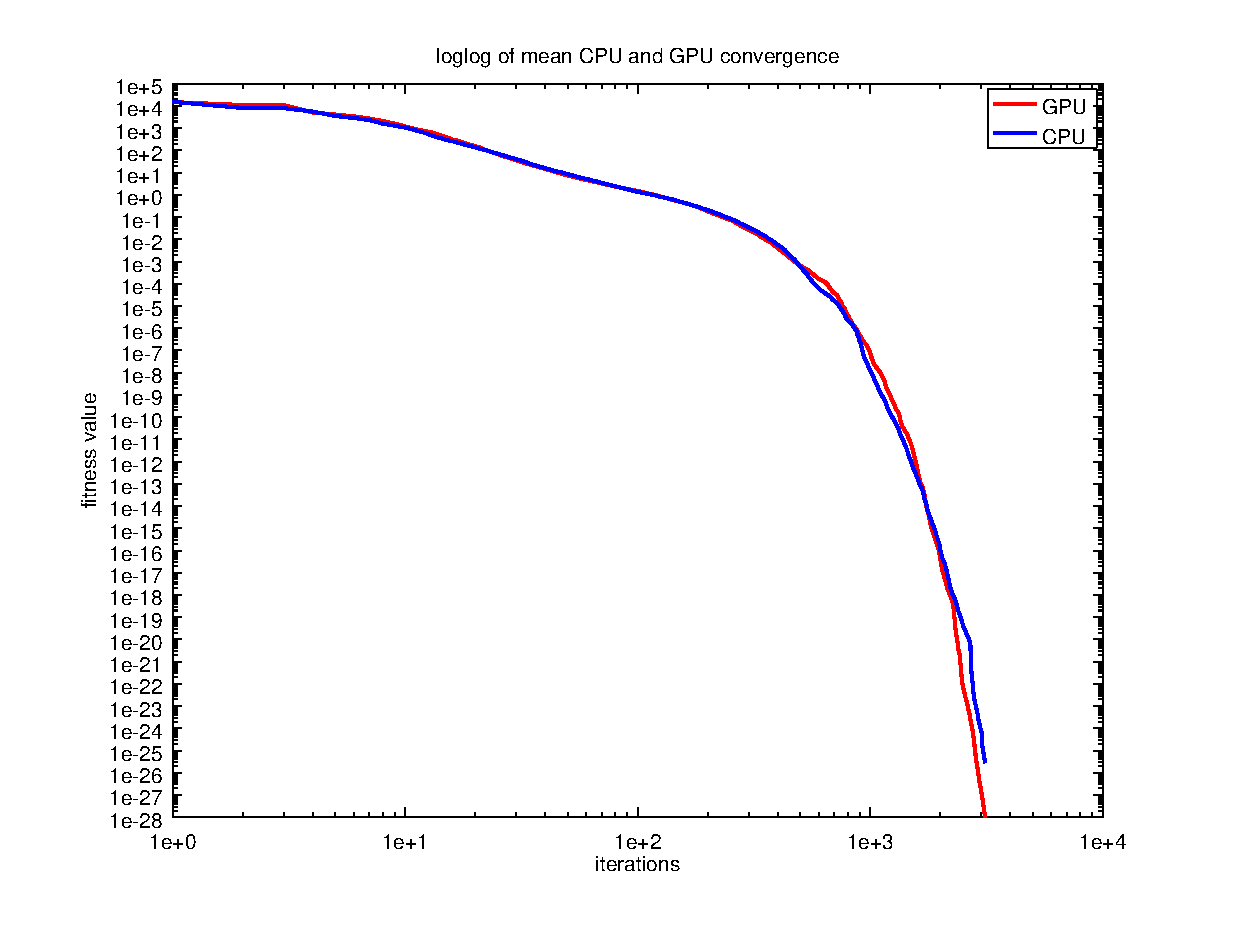
\includegraphics[width=.7\textwidth]{../img/loglog_convergence.eps}
        \caption{loglog of mean CPU and GPU convergence}
        \label{fig:loglog_convergence}
    \end{figure}

    \begin{figure}[!htb]
        \centering
        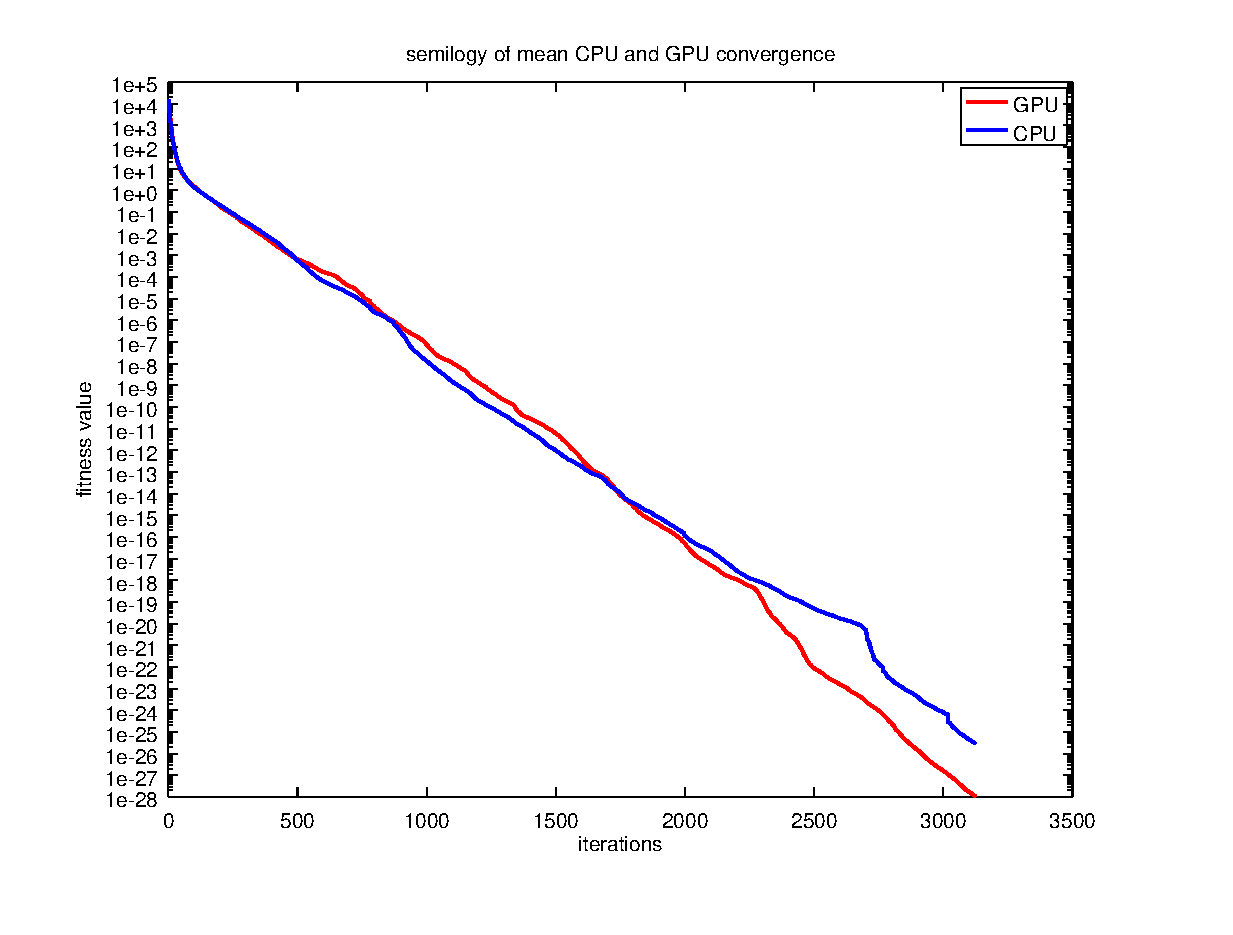
\includegraphics[width=.7\textwidth]{../img/semilogy_convergence.eps}
        \caption{semilogy of mean CPU and GPU convergence}
        \label{fig:semilogy_convergence}
    \end{figure}

    Then, we implemented a version using shared memory also.
    The best-known fitness, the previous best, the population (or swarm), the fitness values and the adjacency matrix use shared memory.
    We compare the three versions (CPU, GPU, and GPU with shared memory). In terms of convergence the results were similar (as they should [Figure~\ref{fig:sphere10_32particles_fitness}]).
    The experiments were repeated $51$ times with the GPU versions using just one block with 32 threads. The GPU with shared memory was faster than GPU without using shared memory. But, the CPU implementation was the fastest (Figure~\ref{fig:sphere10_32particles_time}).


    \begin{figure}[!htb]
        \centering
        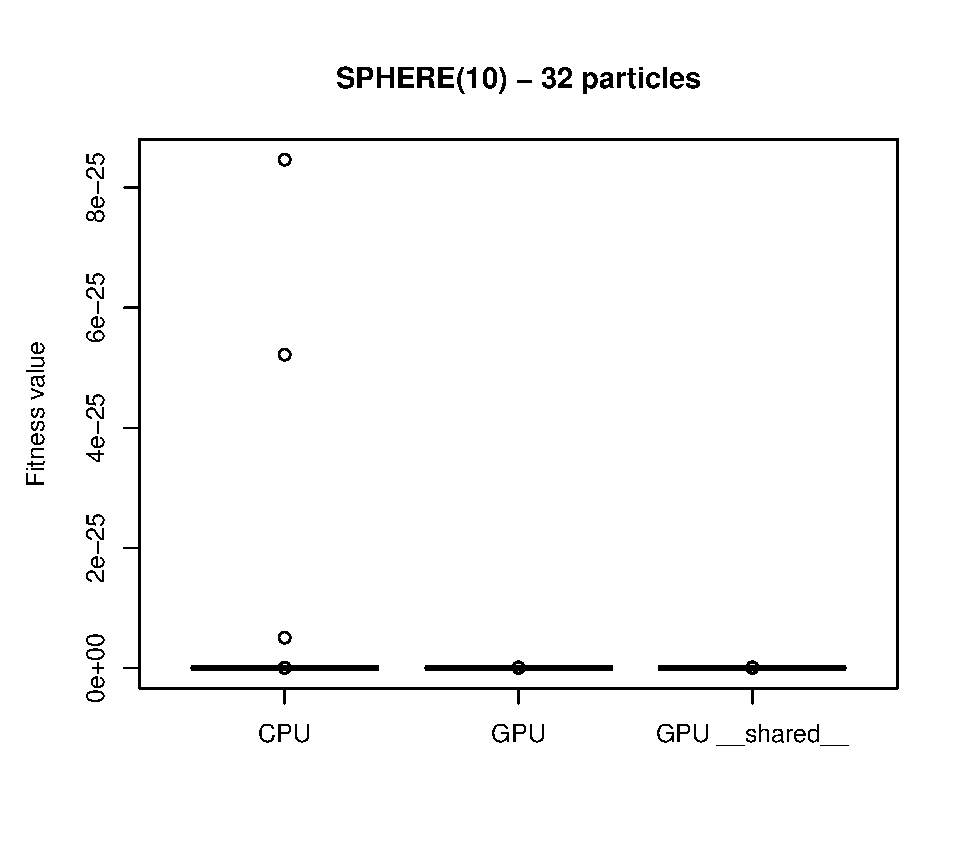
\includegraphics[width=.7\textwidth]{../img/sphere10_32particles_fitness.eps}
        \caption{Convergence of different implementations (single block - 51 executions)}
        \label{fig:sphere10_32particles_fitness}
    \end{figure}


    \begin{figure}[!htb]
        \centering
        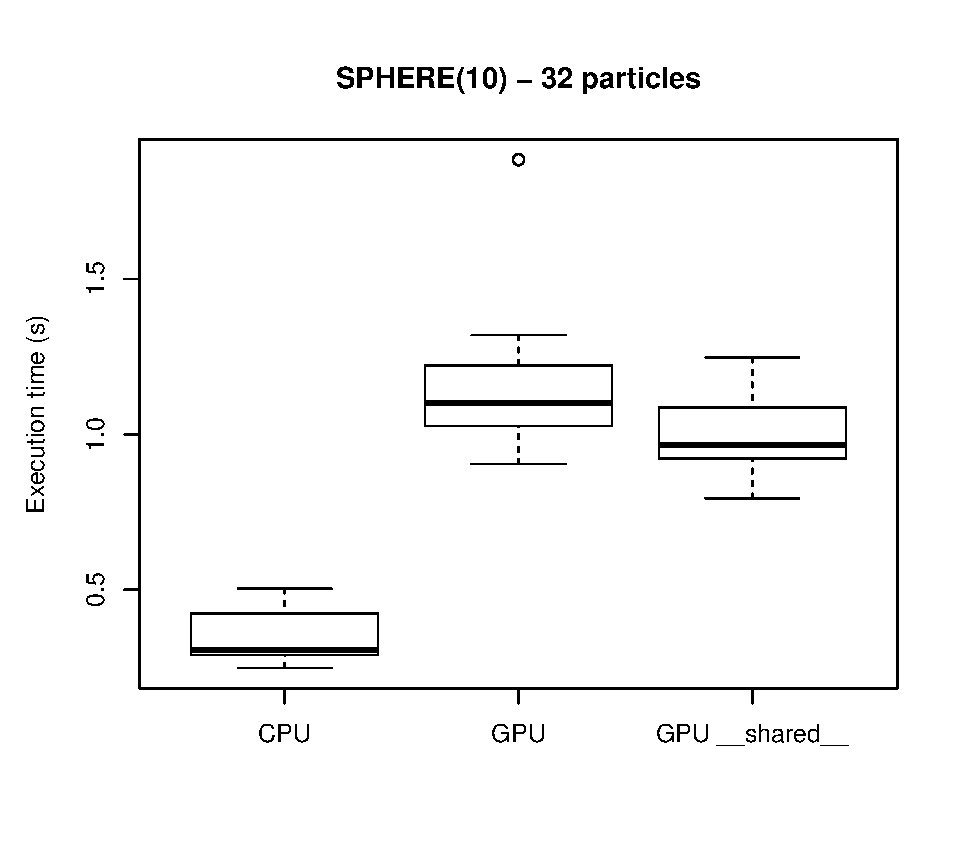
\includegraphics[width=.7\textwidth]{../img/sphere10_32particles_time.eps}
        \caption{Execution time of different implementations (single block - 51 executions)} 
        \label{fig:sphere10_32particles_time}
    \end{figure}


    To use the CUDA parallelism capabilities and exploit the characteristics of SPSO the GPU implementation executes the $51$ runs in parallel using 51 blocks. To evaluated the execution time we repeat the experiment30 times. The fitness of the GPU (with shared memory) and CPU continued to be similar (Figure~\ref{fig:sphere10_32particles_multi_runs_fitness}) but the execution time of the GPU was faster than CPU (Figure~\ref{fig:sphere10_32particles_multi_runs_time}).

    \begin{figure}[!htb]
        \centering
        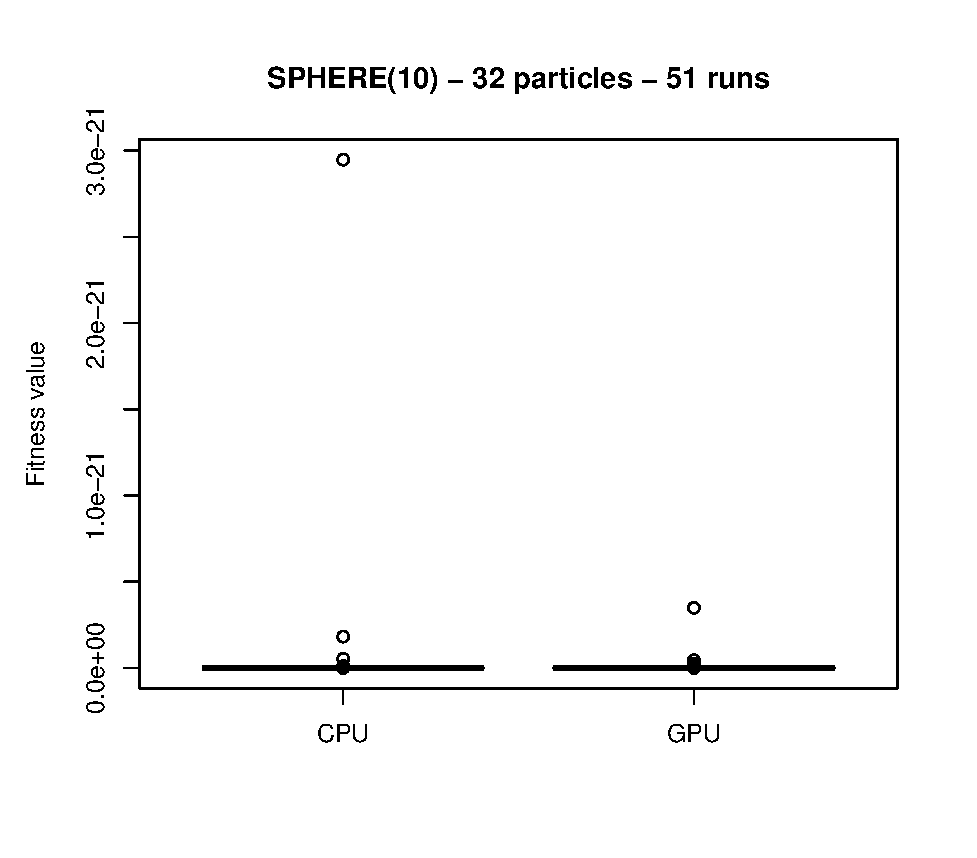
\includegraphics[width=.7\textwidth]{../img/sphere10_32particles_multi_runs_fitness.eps}
        \caption{Convergence of different implementations (GPU 51-blocks, 30 repetitions)}
        \label{fig:sphere10_32particles_multi_runs_fitness}
    \end{figure}


    \begin{figure}[!htb]
        \centering
        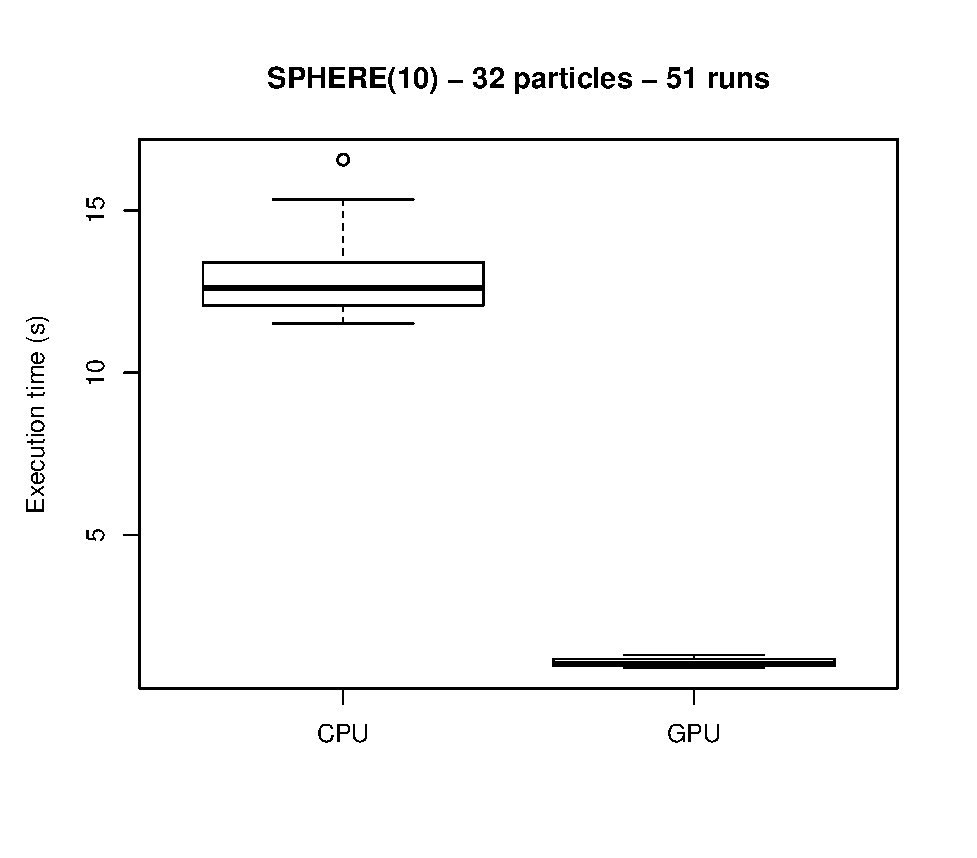
\includegraphics[width=.7\textwidth]{../img/sphere10_32particles_multi_runs_time.eps}
        \caption{Execution time of different implementations (GPU 51-blocks, 30 repetitions)}
        \label{fig:sphere10_32particles_multi_runs_time}
    \end{figure}

    \section{Conclusions}

    In this project, we implement a Parallel Standard Particle Swarm Optimization.
    First, we compare the implementations regarding convergence quality, in which both GPU and CPU implementations were similar.
    After different implementations and experiments, it was possible to achieve a 12.054 speed up. The execution time of the CPU version for 51 runs was 12.84892 seconds (in an average of 30 repetitions). Moreover, the execution time for the GPU version was 1.065946 seconds.

    \bibliographystyle{plain}
    \bibliography{bibliography} 

\end{document}
